\documentclass[fleqn]{latex-classes/summary}

\title{Notizen zur ML-Klausur}
\author{Jens Ochsenmeier}

\begin{document}

\section*{Hinweise aus letzter Vorlesung}

\paragraph{Themen, die besonders wichtig sind}

\begin{itemize}
  \item \textbf{Lerntheorie}
  \item \textbf{SVM}
  \begin{itemize}
    \item Basisprinzip: Expertenwissen, um SVM anzuwenden (Merkmalsraum kann kompliziert werden)
    \item Erweiterung auf nichtlineare Probleme: siehe Beispiel aus Vorlesung (Klassifikation)
    \item Merkmalsraum \( \leftrightarrow \) Hypothesenraum
  \end{itemize}
  \item \textbf{Neuronale Netze}
  \begin{itemize}
    \item Basisprinzip
    \item Fehlerfunktion und Fehler ableiten
    \item Gradientenabstieg \( \to \) Parameter anpassen
    \item Aufbau Neuron
    \item Aktivierungsfunktionen
  \end{itemize}
  \item \textbf{Faltungsnetze}
  \begin{itemize}
    \item Kerne, mit denen gefaltet wird (scheinbar nicht wirklich wichtig)
    \item Schichten und Kerne: Aufbau
    \item Dimensionen von Featuremaps: Veränderungen, Methoden
    \item Max-Pooling
    \item Verbindung von CNNs
  \end{itemize}
  \item \textbf{Entscheidungsbäume}
  \begin{itemize}
    \item Aufbau
    \item Bestimmung von Attributen (\emph{information gain})
  \end{itemize}
  \item \textbf{Sum-Product-Netze}
  \begin{itemize}
    \item Wann ist SPN gültig?
    \item SPN Verteilung, Scopes?
    \item Mit Regeln testen, ob es passt
    \item Kleine Beispiele kennen
    \item Lernansätze (zB Parameterlernen, Strukturlernen mit vollständig beobachteten Daten)
    \item[\( \to \)] vor allem grundsätzliche Methoden
  \end{itemize}
  \item \textbf{Reinforcement Learning}
  \begin{itemize}
    \item Was heißt das?
    \item Markovsche Entscheidungsfunktion und andere Funktionen
    \item An kleinem Beispiel durchrechnen
  \end{itemize}
  \item \textbf{Bayessches Lernen}
  \begin{itemize}
    \item Bedingte Abhängigkeiten
    \item Bayes-Ansatz durchrechnen
    \item Annahmen (zB naive Bayes-Annahme)
    \item Wohin führt Berechnung?
  \end{itemize}
\end{itemize}

\paragraph{Weitere Tipps}

\begin{itemize}
  \item Definition VC-Dimension kennen (hängt von Topologie ab), zusammen mit CNNs \\*
    \( \to \) Anzahl Neuronen in Topologie lässt Schlüsse auf VC zu
  \item Zöllner hat paar Aufgaben von WS17/18 gezeigt, will aber nicht alles zeigen, \textbf{weil einiges ähnlich ist!}
  \item Altklausur 3e: VC-Dimension zu groß, es gibt Overfitting \\*
    \( \to \) Verbesserung: Anpassen der VC-Dim oder der Kapazität (verringern), mehr Beispiele
  \item Altklausur 3f: cascade correlation
  \item Aufgabe zu Q-Algorithmus wurde gezeigt, aber nicht im Detail auf Folien. Allerdings \textbf{V-Algorithmus} durchrechnen ``ist auch recht wichtig'' \\*
    \( \to \) Berechnung zu V-Algorithmus kommt höchstwahrscheinlich dran
  \item Ergebnisse reichen, aber Bellmann-Gleichung schadet nicht
  \item Bei Wahrscheinlichkeiten: Aufgabenstellung beachten! Arithmetischer Ausdruck reicht oftmals
  \item Gradienten: Verwendung
  \item Boosting und Bagging mit anderen Verfahren
\end{itemize}

\newpage

\section*{Altklausur WS17/18}

\paragraph{Aufgabe 1 -- Allgemeine Fragen}

\begin{enumerate}
  \item Geben Sie 3 Einordnungskriterien von Lernverfahren, sowie deren Abstufungen bzw. Ausprägungen an.
  \item Beschreiben Sie das Problem des \textbf{Overfitting}. Wie kann es verhindert werden?
  \item Was verbirgt sich hinter der \textbf{Vapnik-Chervonenkis-Dimension}? Beschreiben Sie den theoretischen Nutzen in der Anwendung.
\end{enumerate}

\paragraph{Aufgabe 2 -- Lernen von probabilistischen Modellen}

\begin{enumerate}
  \item Der folgende Datensatz beschreibt Beobachtungen des Status eines bestimmten Zuges an einem bestimmten Bahnhof gegeben der ebenfalls beobachteten Attribute: \( \text{Tag (T)} \in \left \{ \text{Wochentag}, \text{Wochenende} \right \} \), \( \text{Wind (Wi)} \in \left \{ \text{Kein}, \text{Leicht}, \text{Stark} \right \} \) und \( \text{Wetter (We)} \in \left \{ \text{Sonne}, \text{Regen}, \text{Wind} \right \} \).
    
  \begin{center}
    \small
    \begin{tabular}{ | c | c | c | c | }
      \hline
      \textbf{Tag (T)} & \textbf{Wind (Wi)} & \textbf{Wetter (We)} & \textbf{Status (S)} \\\hline
      Wochentag & Kein & Sonne & Verspätet \\\hline
      Wochentag & Kein & Nebel & Verspätet \\\hline
      Wochentag & Stark & Regen & Pünktlich \\\hline
      Wochenende & Leicht & Regen & Verspätet \\\hline
      Wochentag & Stark & Sonne & Pünktlich \\\hline
      Wochenende & Stark & Nebel & Pünktlich \\\hline
      Wochenende & Kein & Sonne & Verspätet \\\hline      
      Wochentag & Leicht & Regen & Pünktlich \\\hline
      Wochenende & Leicht & Nebel & Verspätet \\\hline
    \end{tabular}
  \end{center}

  Berechnen Sie folgende (a-priori und bedingte) Wahrscheinlichkeiten:
  \begin{itemize}
    \item \( P(S = \text{Verspätet}) = \)
    \item \( P(S = \text{Pünktlich}) = \)
    \item \( P(T = \text{Wochenende} \mid S = \text{Pünktlich}) = \)
  \end{itemize}

  \item Heute ist ein Wochentag mit Nebel und leichtem Wind. Ein naiver Bayes-Klassifikator soll genutzt werden, um den Status des Zuges vorherzusagen. Welches ist heute der wahrscheinlichste Status des Zuges? Begründen Sie Ihre Entscheidung.

  \item Das Szenario aus der vorherigen Teilaufgabe wird nun zusätzlich um das Attribut Jahreszeit (\( J \)) erweitert. Folgende Abhängigkeiten zwischen den Attributen sind gegeben:
  \begin{itemize}
    \item Wetter (We) und Wind (Wi) sind abhängig von der Jahreszeit (J)
    \item Der Status (S) ist abhängig von Wetter (We), Wind (Wi) und Tag (T)
  \end{itemize}
  Zeichnen Sie ein Bayessches Netz, welches das Szenario beschreibt.

  \item Was kann bei einem Bayesschen Netz gelernt werden? Mit welcher Methode erfolgt dies, wenn die Struktur bekannt ist und Variablen nur teilweise beobachtbar sind?
  
  \item Ein HMM (\emph{hidden markov model}) ist definiert als
  
  \begin{align*}
    \lambda = \{ &S \text{ -- Zustände}, \\
    &V \text{ -- Ausgabezeichen}, \\
    &A \text{ -- Übergangswahrscheinlichkeiten}, \\
    &B \text{ -- Emmisionswahrscheinlichkeiten}, \\
    &\Pi \text{ -- Verteilung Anfangswahrscheinlichkeiten} \}\text{.}
  \end{align*}
  Beschreiben Sie das Lernproblem (was ist gegeben?, was ist gesucht?). Welcher Lernansatz kann dafür verwendet werden und welche Parameter werden dabei gelernt?
\end{enumerate}

\newpage

\paragraph{Aufgabe 3 -- Neuronale Netze}

\begin{enumerate}
  \item Ergänzen Sie fehlende Begriffe und Formeln in der untenstehenden Abbildung eines Neurons.
  \begin{figure}[H]
    \centering
    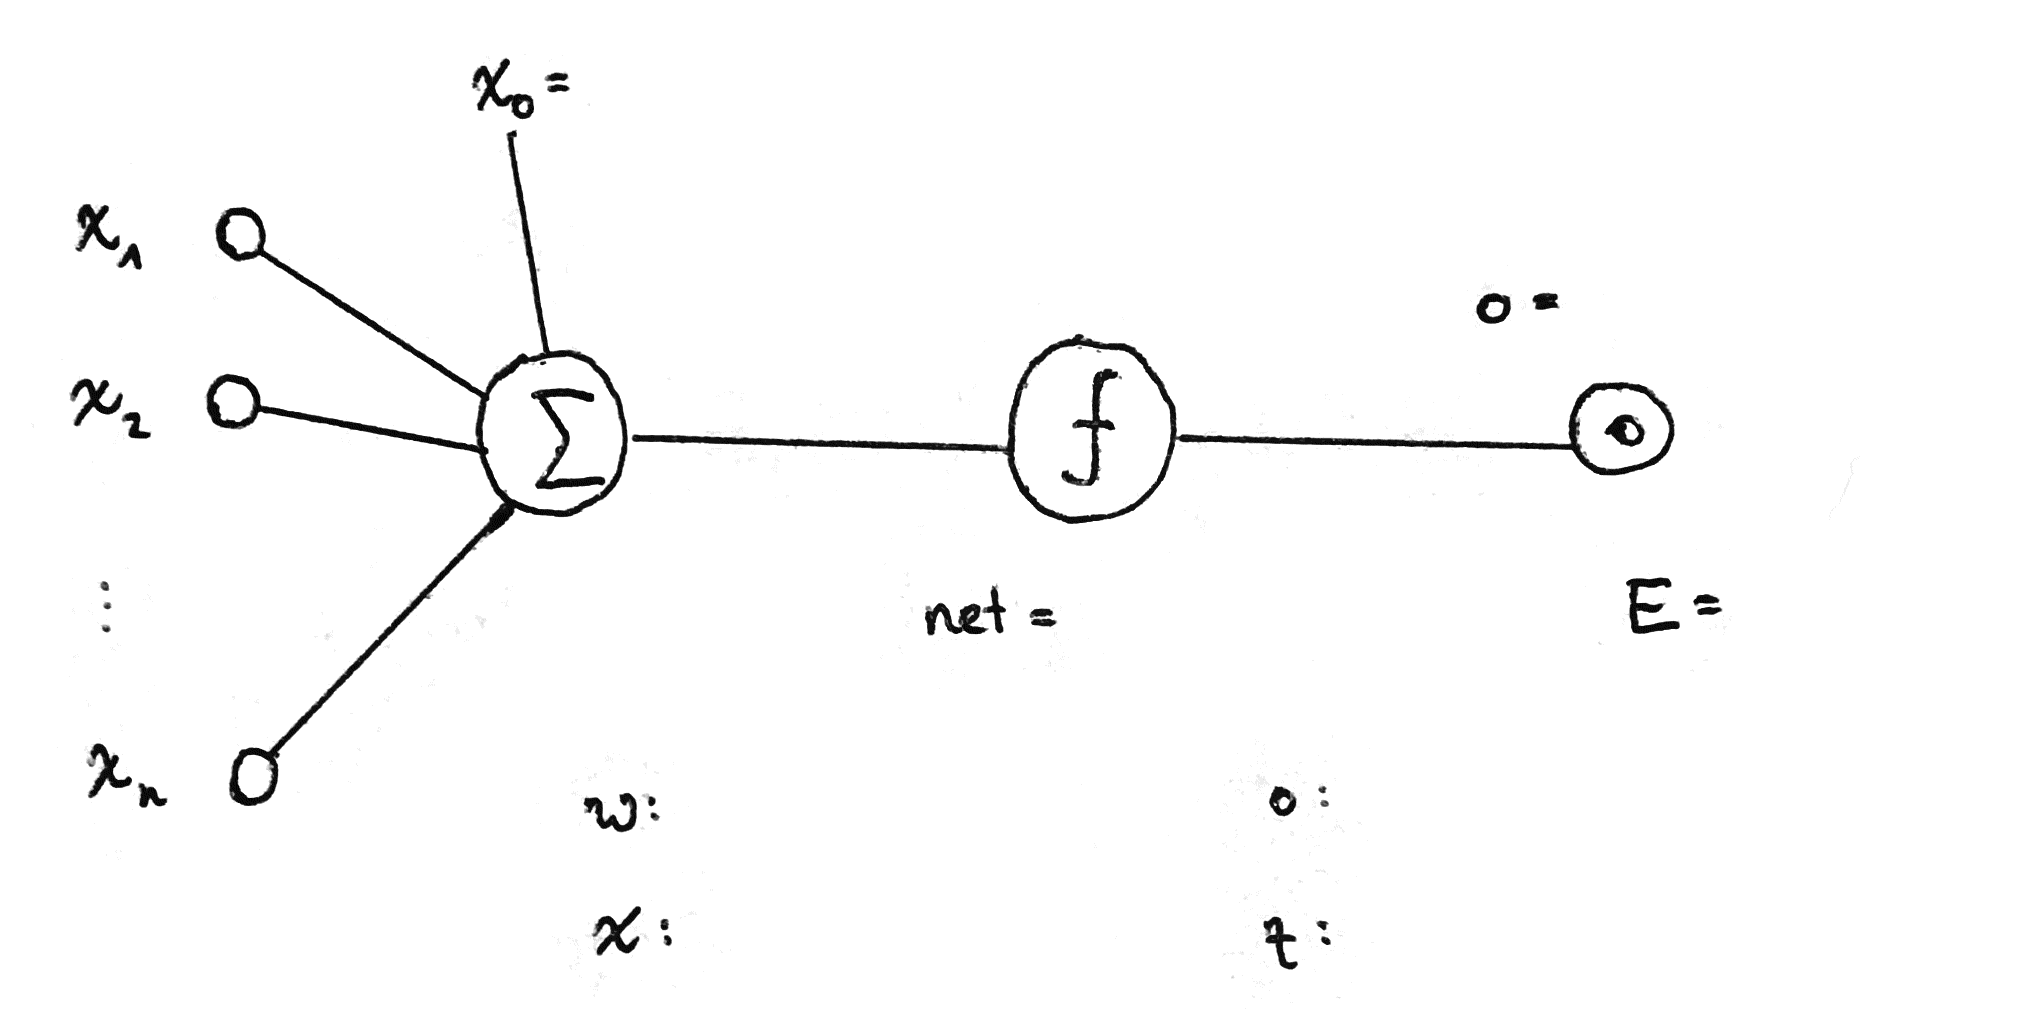
\includegraphics[width=.8\linewidth]{assets/img/neuron.png}
  \end{figure}

  \item Nennen Sie zwei typische nichtlineare Aktivierungsfunktionen, die jeweils dazugehörige Formel und die jeweiligen Ableitungen.
  \item Welche Bedingung muss die Aktivierungsfunktion eines Neurons für das Lernen unter Verwendung des Gradientenabstiegs erfüllen?
  \item Nennen Sie ein Lernverfahren, um vorwärts gerichtete, mehrschichtige neuronale Netze zu trainieren und eine Herausforderung, die beim involvierten Gradientenabstieg auftreten kann. Mit welcher Methode kann dabei das Lernen verbessert werden?
  \item Was lässt sich über die VC-Dimension des neuronalen Netzes sagen, das aus den untenstehenden Lerndaten die eingezeichnete Kurve approximiert? Nennen Sie das resultierende Phänomen und beschreiben Sie kurz, wie sich die Approximation verbessern lässt.
  \begin{figure}[H]
    \centering
    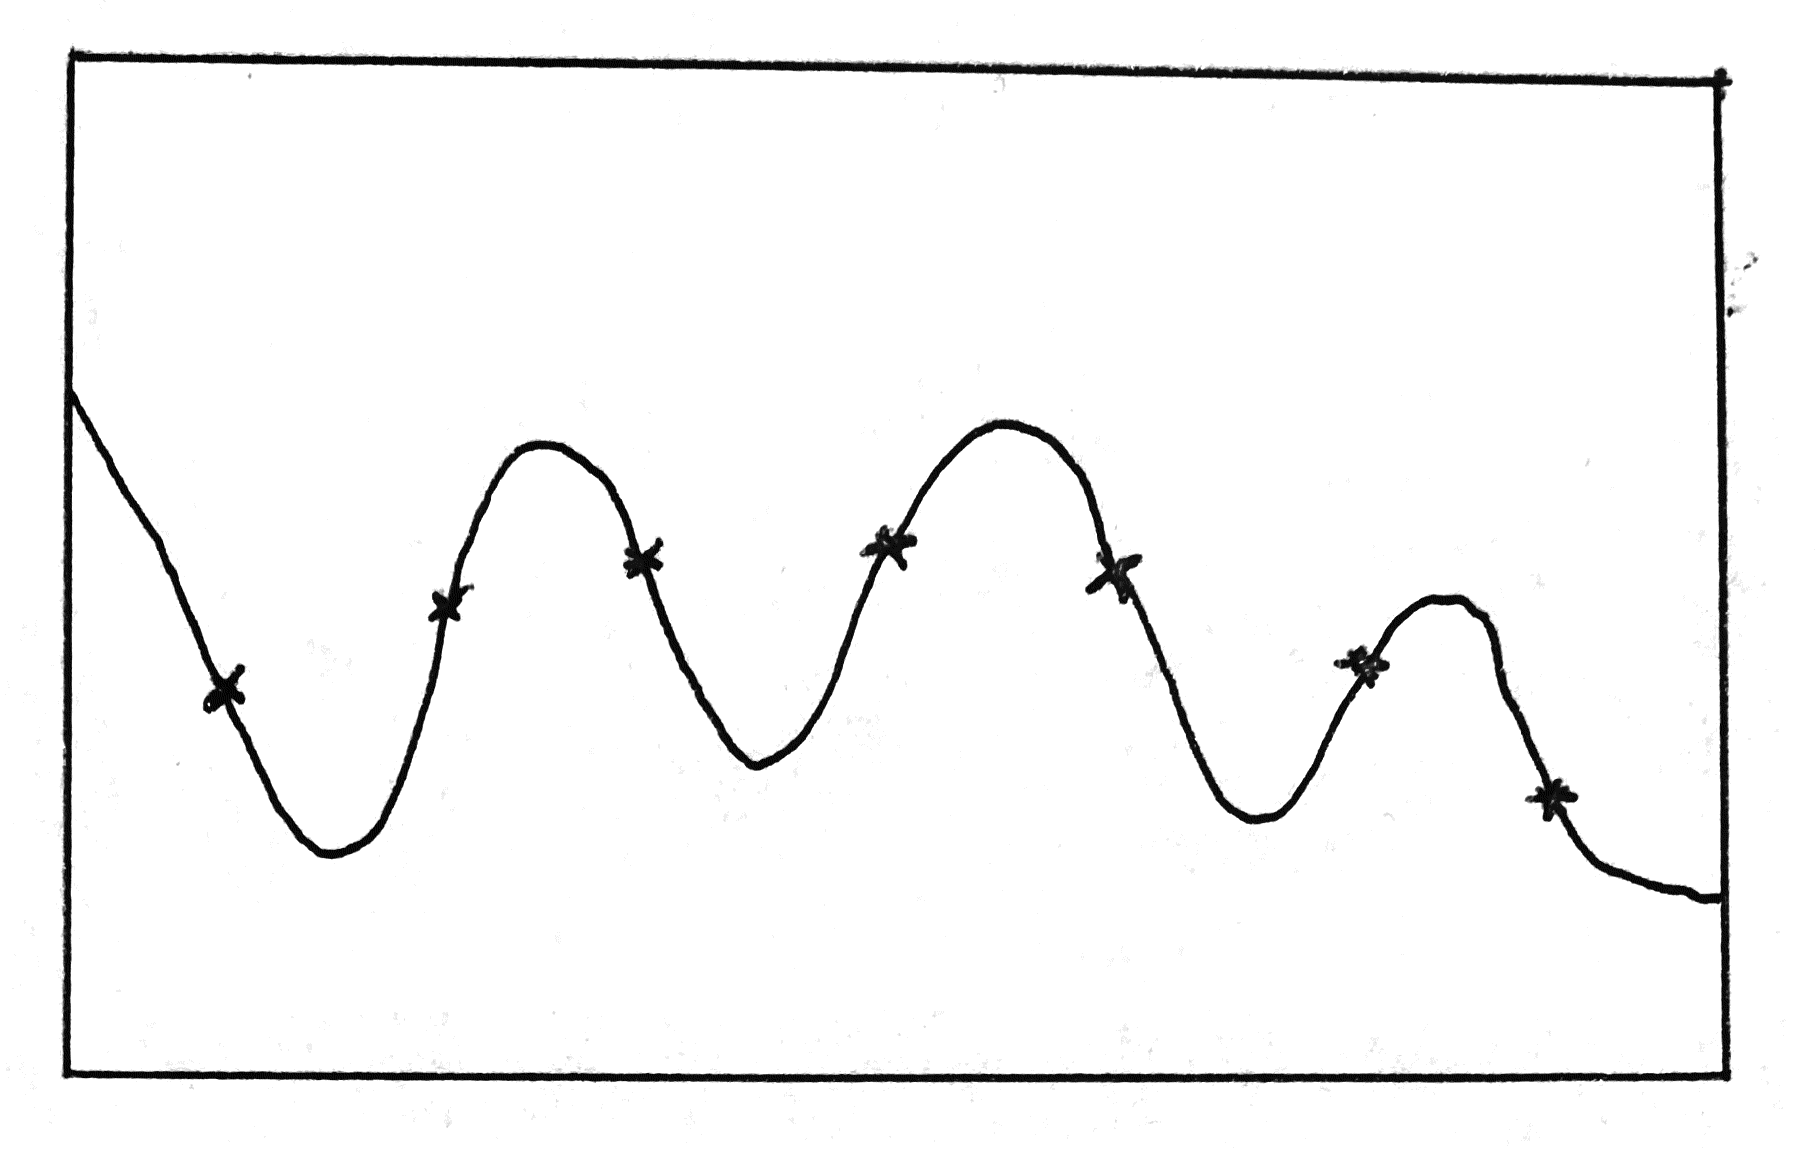
\includegraphics[width=.5\linewidth]{assets/img/vc.png}
  \end{figure}

  \item Nennen Sie ein konstruktives Verfahren zur schrittweisen Optimierung der Netzwerktopologie.
\end{enumerate}

\paragraph{Aufgabe 4 -- Reinforcement Learning}

\begin{enumerate}
  \item Durch welches Modell lässt sich die Problemstellung beim Reinforcement Learning formal darstellen? Welche vier Bestandteile werden für die Modellierung benötigt?
  \item Beschreiben Sie kurz die Markov-Bedingung.
  \item Wie lautet die rekursive Definition der Q-Funktion (Bellmann-Gleichung)?
  \item Nennen Sie die zwei wesentlichen Unterschiede zwischen den Suchstrategien \emph{Exploration} und \emph{Eploitation}.
  \item Betrachten Sie das untenstehende Labyrinth. Ein Agent kann sich mit den angezeigten Zustandsübergängen von Raum zu Raum bewegen. Der Reward für einen Übergang ist jeweils in der Zeichnung abgebildet. Zu Beginn des Trainings gilt \( \forall s, a : Q(s,a) = 0 \). Führen Sie den Q-Learning-Trainingsalgorithmus durch und tragen Sie die Schätzung \( \hat{Q}(s,a) \) für alle \( (s,a) \) nach konvergieren des Lernalgorithmus (Diskontierungsfaktor \( \gamma = 0.8 \)) ein. Runden Sie die Ergebnisse auf natürliche Zahlen.
  
  \begin{figure}[H]
    \centering
    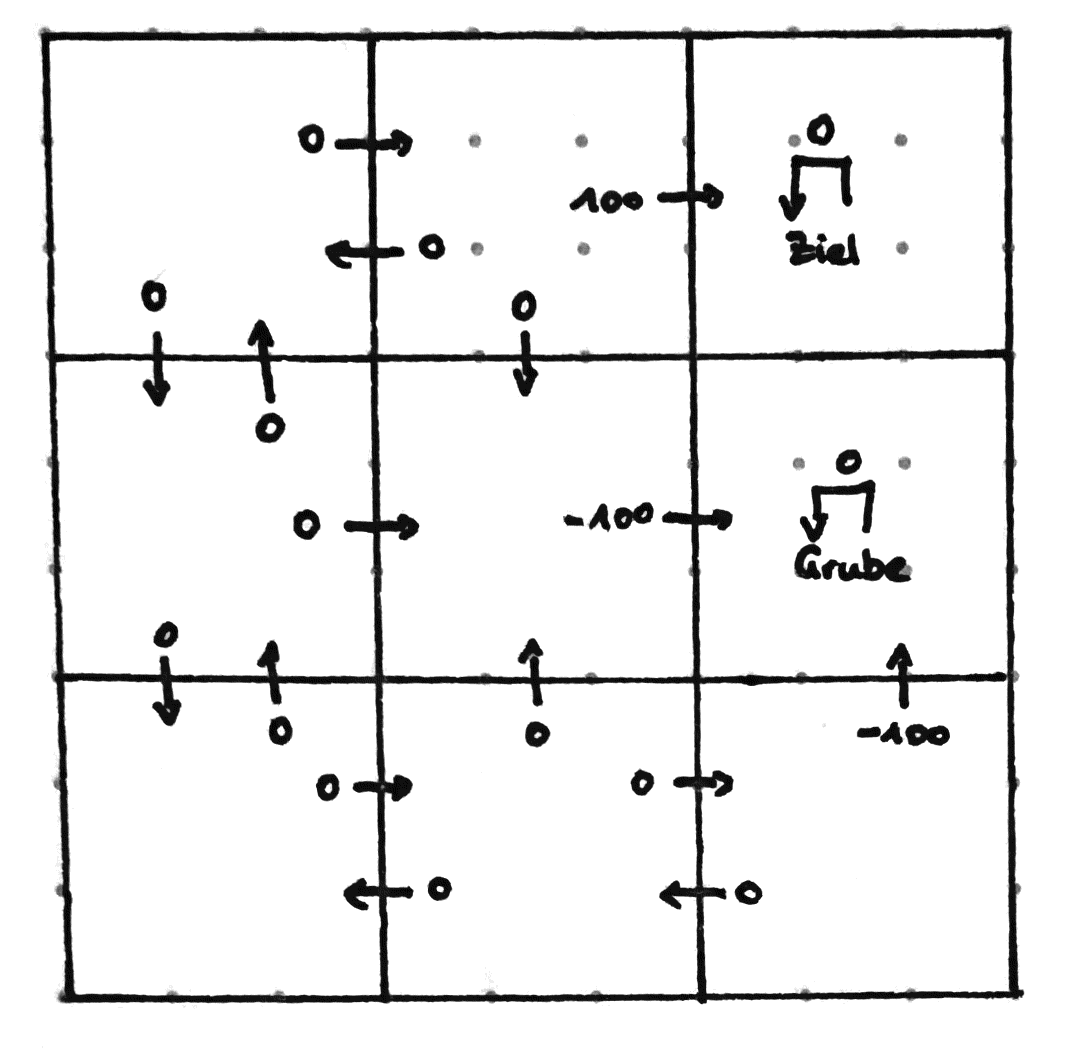
\includegraphics[width=.6\linewidth]{assets/img/q.png}
  \end{figure}
\end{enumerate}

\newpage

\paragraph{Aufgabe 5 -- Boosting}

Mit Hilfe von AdaBoost soll eine Klassifizierung durchgeführt werden. Hieru soll ein Entscheidungsstumpf (1-Merkmals-Entscheidungsbaum mit lediglich einer Wurzel und zwei Blättern) verwendet werden. In jeder Iteration wählen Sie den Stumpf, der den gewichteten Trainingsfehler minimiert. Nutzen Sie hierzu die untenstehende Zeichnung.

\begin{figure}[H]
  \centering
  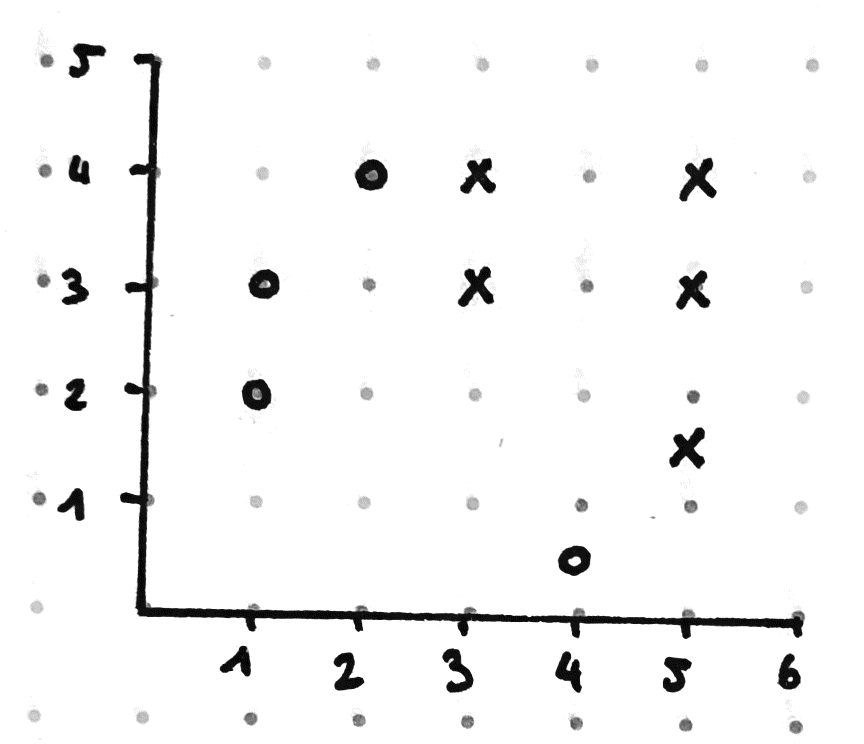
\includegraphics[width=.4\linewidth]{assets/img/adaboost.png}
\end{figure}

\begin{enumerate}
  \item Zeichnen Sie die Entscheidungsgerade in die obige Abbildung ein. Markieren Sie die positive und negative Seite der Klassifikation.
  \item Berechnen Sie die Gewichtung jedes Datenpunktes nach der ersten Iteration und markieren Sie den Datenpunkt, der die höchste Gewichtung nach der ersten Iteration besitzt.
  \item Erklären Sie anhand von AdaBoost die Anwendung der strukturellen Risikominimierung. Gehen Sie dabei auf die wesentlichen Aspekte der Hypothesenraumstrukturierung und der Fehlerminimierung ein.
\end{enumerate}

\paragraph{Aufgabe 6 -- Support Vector Machines}

\begin{enumerate}
  \item Beschreiben Sie kurz die Grundidee, die der Methode der Support-Vektor-Klassifikation zugrunde liegt und wie das Verfahren einzuordnen ist.
  \item Geben Sie die Formeln für das Optimierungskriterium der \textbf{optimalen} Hyperebene und für die Randbedingung einer korrekten Klassifikation an (gegeben Trainingsbeispiele der Form \( (\overrightarrow{x}, y) \)).
  \begin{itemize}
    \item Optimierungskriterium:
    \item Randbedingung:
  \end{itemize}
  \item Erklären Sie die Dualität zwischen Hypothesenraum und Merkmalsraum im Kontext des SVM-Verfahrens (\emph{version space duality}).
  \item Welche Vorteile ergeben sich durch den sogenannten ``Kerneltrick''? Welche Beobachtung liegt dem Kerneltrick zugrunde?
\end{enumerate}

\end{document}